\documentclass[conference]{IEEEtran}
\usepackage{cite}
\usepackage{amsmath,amssymb,amsfonts}
\usepackage{graphicx}
\usepackage{booktabs}
\usepackage{multirow}
\usepackage{algorithm}
\usepackage{algpseudocode}
\usepackage{xcolor}
\usepackage{url}
\usepackage{tikz}
\usetikzlibrary{arrows.meta,positioning,shapes.geometric,fit,backgrounds}
\graphicspath{{figures/}}

\begin{document}

\title{An Explainable Freeway Congestion Prediction Agent Grounded in Real-World ETC Data and Official Traffic Regulations}

% TODO: Replace with author name(s) and institutional email(s).
\author{\IEEEauthorblockN{First Author and Second Author}
\IEEEauthorblockA{Department of Computer Science and Engineering\\
National Chung Hsing University\\
Taichung, Taiwan\\
Email: author@example.com}}

\maketitle

\begin{abstract}
Severe holiday congestion on Taiwan's National Freeway No.~5 remains a persistent challenge for pre-trip planning; during the 2026 Lunar New Year peak period, daily average freeway traffic volume reached 124.0 million vehicle-kilometers, approximately $1.3\times$ the weekday annual average. Although traffic speed forecasting models and mobile navigation services exist, a substantial gap remains between raw predictive accuracy and actionable, evidence-based travel advice. Existing forecasting studies primarily output numerical speeds without regulatory context, official platforms do not publish auditable accuracy benchmarks, and emerging large language model (LLM) traffic agents risk numerical hallucination when reasoning directly over traffic figures. To address these challenges, we propose an explainable freeway congestion prediction agent that treats machine learning models and an official traffic regulation knowledge base as programmatic tools. Numerical speed forecasting, conditional isotonic probability calibration, regulatory matching, and departure-timing rules are executed deterministically in code, while an LLM handles natural-language query parsing and explanation under strict numerical-grounding verification and automatic template fallback. Built on Taiwan's Electronic Toll Collection (ETC) TDCS M05A gantry data and aligned real-time XML feeds across the ten mainline segments of National Freeway No.~5, the system predicts traffic speeds and calibrated congestion risks 15, 30, and 60 minutes ahead while distinguishing zero-flow missingness from true congestion. Models trained on 2024 data are evaluated on full-year 2025 data and 311 out-of-sample days in 2026 against persistence and historical-average baselines using day-level clustered bootstrap confidence intervals, matched-budget event-level detection, calibration diagnostics, delay sensitivity, and a SHA-256-frozen 72-query agent benchmark. Results show that gradient-boosted regression consistently lowers speed MAE relative to persistence on workdays ($-0.36$ to $-0.75$~km/h) and regular weekends ($-0.31$ to $-0.70$~km/h), whereas multi-day holiday gains remain small and unstable across years ($-0.04$~km/h at 60~min in 2026) and event-level early warning does not outperform persistence. Meanwhile, the agent achieves 100\% numerical grounding, scope enforcement, and announcement citation across all 72 test cases, demonstrating the practical value of verifiable tool-first agent design.
\end{abstract}

\begin{IEEEkeywords}
Congestion prediction, explainable artificial intelligence, intelligent transportation systems, large language models, traffic speed forecasting.
\end{IEEEkeywords}

\section{Introduction}

\subsection{Background and Motivation}
Intercity highway congestion during weekends and multi-day public holidays poses significant economic and commuter burdens worldwide. In Taiwan, National Freeway No.~5 (the Chiang Wei-shui Freeway connecting Taipei's Nangang System to Su'ao via the 12.9~km Hsuehshan Tunnel) is a prominent bottleneck corridor where northbound return flows routinely back up between Yilan and Pinglin. According to official statistics from Taiwan's Freeway Bureau (Ministry of Transportation and Communications, MOTC), daily average freeway traffic volume during the 2026 Lunar New Year peak period (Day~1 to Day~6) reached 124.0 million vehicle-kilometers, approximately $1.3\times$ the weekday annual average of 93 million vehicle-kilometers~\cite{freeway2026cny}. Real-world observations corroborate this severity, with mainline speeds between Yilan and Toucheng dropping as low as 14~km/h during peak holiday waves (e.g., May~31, 2025).

At the same time, Taiwan's Electronic Toll Collection (ETC) infrastructure publishes open 5-minute gantry-to-gantry median speed and volume archives through the Traffic Data Collection System (TDCS M05A) alongside real-time XML feeds (\texttt{ETagPairLive.xml} and \texttt{LiveEvents.xml})~\cite{tdcs_m05a}. These public roadside streams create an opportunity to move beyond static dashboards toward interactive, evidence-backed pre-trip decision support.

\subsection{Problem Statement}
Despite rapid progress in traffic forecasting and conversational artificial intelligence, translating freeway speed forecasts into trustworthy pre-trip advice faces four interrelated obstacles:
\begin{enumerate}
    \item \emph{Accuracy--Utility Gap}: Most academic forecasting models emit raw numerical speeds or travel times without explaining model uncertainty, data freshness, or applicable traffic control policies such as high-occupancy vehicle (HOV) restrictions and entrance ramp closures.
    \item \emph{Opaque Operational Benchmarks}: Official traveler services such as the Freeway 1968 App provide real-time conditions and travel-time estimates, yet do not disclose reproducible accuracy metrics, calibration diagnostics, or auditable evidence traces for pre-trip recommendations.
    \item \emph{LLM Numerical Unreliability}: Recent LLM-based transportation assistants largely focus on simulation control or database querying; when asked to interpret predictions directly, LLMs frequently hallucinate unsupported numbers, omit mandatory caveats, or conflate forecasting limitations with official policies.
    \item \emph{Data-Quality Pitfalls in Roadside ETC Feeds}: In raw M05A and live ETag records, segments with zero passing vehicles are logged with both speed $= 0$ and volume $= 0$. Treating such zero-flow intervals as 0~km/h traffic jams severely distorts both training labels and real-time congestion alerts.
\end{enumerate}

\subsection{Research Objectives}
This study aims to design, implement, and rigorously evaluate a domain-specific, explainable congestion prediction agent for Taiwan's National Freeway No.~5 mainline (10 directional segments) over 15-, 30-, and 60-minute horizons. Rather than attempting to replace official navigation apps or claim state-of-the-art forecasting superiority, our objective is to determine whether predictive modeling, data-quality verification, official regulatory retrieval, and explicit limitation disclosure can be unified in a single auditable workflow where every numerical claim is programmatically verified.

\subsection{Research Contributions}
The main contributions of this work are threefold:
\begin{itemize}
    \item \textbf{Tool-First Explainable Traffic Agent with Anti-Hallucination Guardrails}: We decouple numerical forecasting, conditional isotonic probability calibration, regulatory knowledge retrieval, and departure-timing rules from LLM language processing. Every LLM-generated response is checked against a structured fact sheet via deterministic numerical verification and required-content auditing, falling back immediately to a rule-based template upon any violation.
    \item \textbf{Data-Quality-Aware Historical and Live ETC Pipeline}: We formalize zero-flow missingness filtering, outlier screening, bounded forward-fill, and a $-3$-minute slot-alignment rule between \texttt{ETagPairLive.xml} and historical M05A records, empirically verified at 100\% exact agreement across 3,418 records.
    \item \textbf{Reproducible Multi-Year Empirical Evaluation with Scientific Transparency}: Using 2024 training data, full-year 2025 test data, and 311 strict out-of-sample days in 2026, we evaluate speed MAE with day-level clustered bootstrap confidence intervals, matched-budget event-level early warning, probability calibration, delay sensitivity, and a SHA-256-frozen 72-query agent benchmark---candidly reporting both reliable workday/weekend gains and the absence of early-warning advantage over persistence.
\end{itemize}

The remainder of this paper is organized as follows. Section~II reviews related traffic forecasting and LLM agent literature and identifies the research gap. Section~III presents the proposed five-module architecture, methodology, mathematical formulation, and core algorithm. Section~IV details the experimental setup, datasets, metrics, empirical results, and discussion of limitations. Section~V concludes the paper and outlines future work.

\section{Related Work}

\subsection{Existing Approaches}
Traffic prediction and intelligent transportation assistance have evolved along three primary trajectories, complemented by operational domain practices.

\subsubsection{Classical Statistical and Machine Learning Methods}
Early short-term traffic forecasting relied on Historical Averages (HA) and linear time-series formulations such as Seasonal ARIMA (SARIMA), which explicitly model weekly periodicities in highway flow~\cite{williams2003sarima}. Nonlinear kernel methods, notably Support Vector Regression (SVR), were successfully applied to highway travel-time prediction in Taiwan~\cite{wu2004svr}. For large tabular traffic datasets with mixed continuous and categorical features, histogram-based Gradient Boosted Decision Trees (GBDT)~\cite{ke2017lightgbm,pedregosa2011sklearn} offer fast CPU-based training and strong accuracy without GPU overhead. When classification outputs are interpreted as risk probabilities, post-hoc calibration techniques such as isotonic regression~\cite{zadrozny2002isotonic} are commonly used to correct tree-ensemble overconfidence.

\subsubsection{Deep Spatio-Temporal Architectures}
With the proliferation of ETC gantry networks, deep learning models have targeted complex spatio-temporal dependencies. On Taiwan's ETC network, Chen and Chen~\cite{chen2021etc} exploited spatiotemporal mobilities of highway flows for travel-time estimation and prediction. To handle longer temporal horizons efficiently, Informer~\cite{zhou2021informer} introduced sparse self-attention for long-sequence forecasting, while Lin et~al.~\cite{lin2024slit} proposed the Short-Term and Long-Term Integrated Transformer (SLIT) and evaluated it directly on Taiwan highway ETC M05A records.

\subsubsection{LLM-Driven Traffic Systems and Agents}
Recent work integrates LLMs into transportation analytics in two ways. First, models such as ST-LLM~\cite{liu2024stllm} and xTP-LLM~\cite{guo2024xtpllm} adapt LLM backbones for spatio-temporal forecasting and natural-language explanations of traffic trends. Second, tool-augmented agent frameworks---including TrafficGPT~\cite{zhang2023trafficgpt}, TP-GPT~\cite{wang2024tpgpt}, and multi-agent IDM-GPT~\cite{yang2025idmgpt}---enable users to query surveillance databases, invoke traffic simulation tools, or perform customized mobility analysis via natural language.

\subsubsection{Operational Domain Systems and Policies}
In Taiwan, the Freeway Bureau publishes TDCS M05A archives, live XML status/event streams, and holiday traffic management measures including northbound HOV restrictions (requiring $\ge 3$ occupants per passenger car) and southbound ramp closures at Shiding and Pinglin~\cite{tdcs_m05a,freeway2026cny}. The official Freeway 1968 App surfaces current corridor conditions and travel-time predictions for public travelers.

\subsection{Limitations of Existing Methods}
Table~\ref{tab:related_work} summarizes representative paradigms alongside their key strengths and limitations. Classical statistical and deep spatio-temporal models focus almost exclusively on point-error minimization (MAE/RMSE) and rarely integrate regulatory policies, live incidents, or explicit data-quality warnings. Furthermore, per-sample classification metrics (e.g., F1 or ROC-AUC) on imbalanced highway data are easily inflated by already-congested intervals and fail to measure whether drivers receive timely \emph{advance} warning before congestion starts. Conversely, existing LLM-based traffic agents prioritize conversational flexibility, SQL querying, or traffic simulation rather than verifiable real-world roadside forecasting; allowing LLMs to synthesize numbers or omit operational caveats introduces hallucination risks unsuitable for safety-adjacent travel advice. Finally, operational apps lack open, reproducible accuracy reports and auditable evidence trails.

\begin{table*}[!t]
\caption{Comparison of Existing Traffic Forecasting, LLM Agent, and Operational Approaches}
\label{tab:related_work}
\centering
\footnotesize
\setlength{\tabcolsep}{4.5pt}
\begin{tabular}{p{2.3cm}p{2.4cm}p{2.7cm}p{2.4cm}p{2.8cm}p{3.0cm}}
\toprule
\textbf{Category / System} & \textbf{Representative Works} & \textbf{Primary Focus} & \textbf{Domain Regulations \& Events} & \textbf{Key Limitations} & \textbf{Evidence \& Reproducibility} \\
\midrule
Classical Statistical \& ML & HA, SARIMA~\cite{williams2003sarima}, SVR~\cite{wu2004svr}, GBDT~\cite{ke2017lightgbm} & Short-term speed / flow / travel time & Not integrated & Outputs raw numbers only; no user interaction or uncertainty caveats & High reproducibility on open datasets; lacks agent workflow \\
\addlinespace[3pt]
Deep Spatio-Temporal Models & Chen et~al.~\cite{chen2021etc}, Informer~\cite{zhou2021informer}, SLIT~\cite{lin2024slit} & Complex spatio-temporal highway forecasting & Not integrated & High compute cost; black-box outputs; rarely benchmarked on onset alerts & Strong point-error benchmarks; limited decision interpretability \\
\addlinespace[3pt]
LLM Traffic Models \& Agents & ST-LLM~\cite{liu2024stllm}, xTP-LLM~\cite{guo2024xtpllm}, TrafficGPT~\cite{zhang2023trafficgpt}, TP-GPT~\cite{wang2024tpgpt}, IDM-GPT~\cite{yang2025idmgpt} & NL querying, simulation control, explainable forecasting & Limited or static context; no verified local policy DB & Risk of numerical hallucination; few real-time roadside guardrails & Variable; often lacks strict numerical-grounding verification \\
\addlinespace[3pt]
Official Operational Service & Taiwan Freeway 1968 App & Real-time status, travel time, public advisories & Official live controls \& incidents & Closed prediction pipeline; no public accuracy or calibration metrics & Production-grade live data; non-auditable for research \\
\addlinespace[3pt]
\textbf{Proposed Agent (This Work)} & \textbf{Freeway No.~5 Explainable Agent} & \textbf{Tool-first speed/risk forecast + verified pre-trip advice} & \textbf{43 verified KB policies + live XML incidents} & \textbf{Scoped to 10 Freeway No.~5 segments; $\le 60$~min horizon} & \textbf{Open code, 40 unit tests, SHA-256 frozen 72-case eval, 2025--2026 CIs} \\
\bottomrule
\end{tabular}
\end{table*}

\subsection{Research Gap}
Synthesizing prior work reveals a clear progression from \emph{Existing Research} $\rightarrow$ \emph{Limitations} $\rightarrow$ \emph{Research Gap}: there is a lack of an open, reproducible freeway decision-support agent grounded in real roadside ETC streams that combines (1) data-quality-aware historical and live ingestion, (2) calibrated multi-horizon risk estimation honestly benchmarked against simple persistence baselines, (3) verifiable retrieval of official traffic regulations and live incidents, and (4) deterministic anti-hallucination guardrails guaranteeing that every number and policy in natural-language advice is traceable to programmatic tool outputs. Our proposed scheme directly targets this gap.

\section{Proposed Scheme}

\subsection{System Architecture}
To translate roadside ETC measurements into verifiable pre-trip advice for National Freeway No.~5, we design a five-module system organized across three architectural layers (Data Layer, Forecasting Engine Layer, and Agent Layer), as illustrated in Fig.~\ref{fig:architecture}.

\begin{figure*}[!t]
\centering
\resizebox{0.96\textwidth}{!}{%
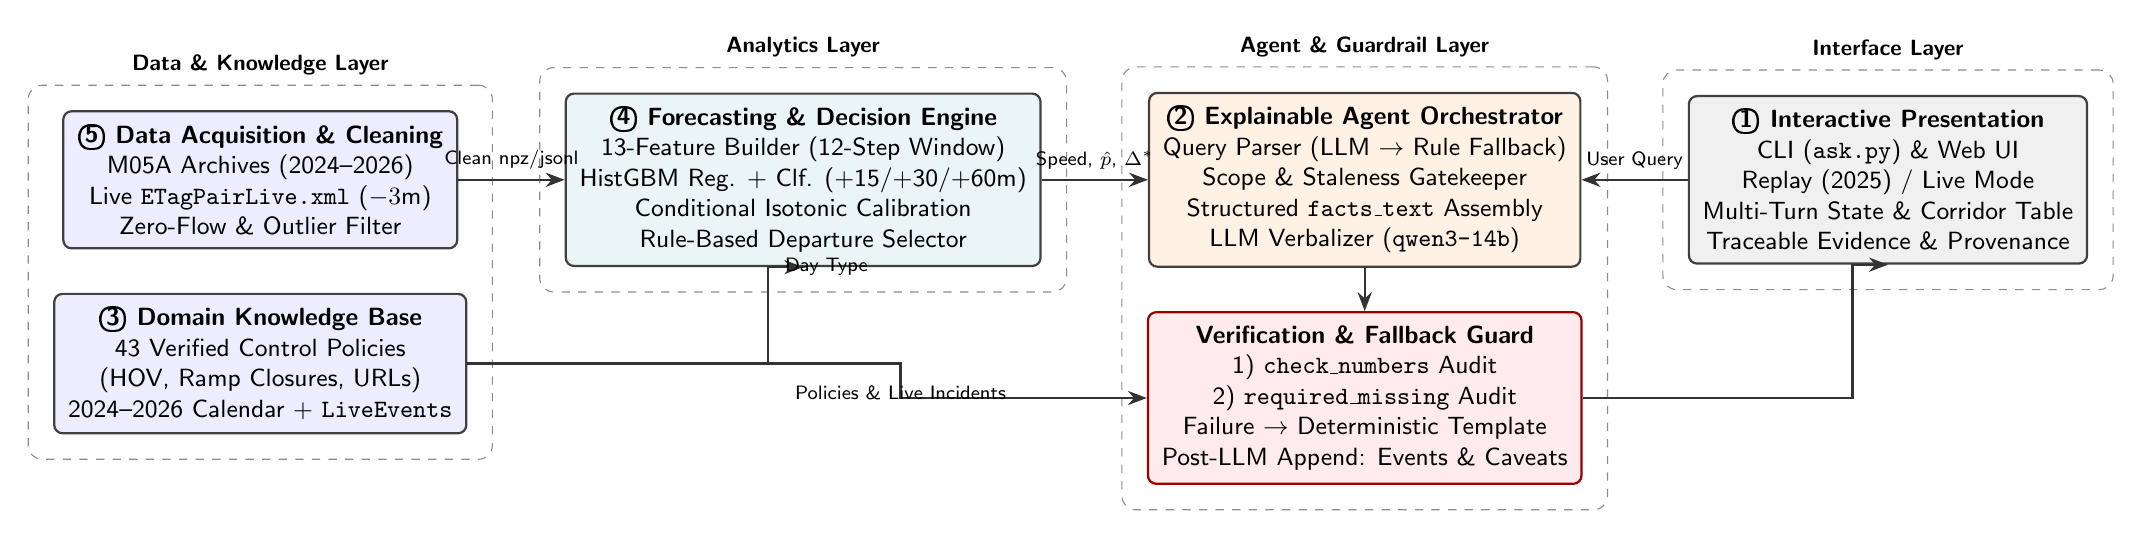
\begin{tikzpicture}[
    font=\sffamily\small,
    node distance=0.6cm and 0.9cm,
    box/.style={rectangle, rounded corners=3pt, draw=black!75, thick, align=center, minimum height=1.05cm, inner sep=5pt},
    data/.style={box, fill=blue!7, minimum width=3.2cm},
    engine/.style={box, fill=teal!8, minimum width=3.5cm},
    agent/.style={box, fill=orange!10, minimum width=3.5cm},
    ui/.style={box, fill=gray!12, minimum width=3.4cm},
    guard/.style={box, fill=red!8, draw=red!60!black, minimum width=3.3cm},
    layer/.style={rectangle, rounded corners=5pt, draw=black!45, dashed, inner sep=9pt},
    arr/.style={-{Stealth[length=2.4mm]}, thick, draw=black!80}
]
% Layer 1: Module 5 & 3 (Data Layer)
\node[data] (m5) {\textbf{\textcircled{5} Data Acquisition \& Cleaning}\\M05A Archives (2024--2026)\\Live \texttt{ETagPairLive.xml} ($-3$m)\\Zero-Flow \& Outlier Filter};
\node[data, below=0.55cm of m5] (m3) {\textbf{\textcircled{3} Domain Knowledge Base}\\43 Verified Control Policies\\(HOV, Ramp Closures, URLs)\\2024--2026 Calendar + \texttt{LiveEvents}};

% Layer 2: Module 4 (Forecasting & Decision Engine)
\node[engine, right=1.35cm of m5] (m4) {\textbf{\textcircled{4} Forecasting \& Decision Engine}\\13-Feature Builder (12-Step Window)\\HistGBM Reg. + Clf. (+15/+30/+60m)\\Conditional Isotonic Calibration\\Rule-Based Departure Selector};

% Layer 3: Module 2 (Agent Orchestrator)
\node[agent, right=1.35cm of m4] (m2) {\textbf{\textcircled{2} Explainable Agent Orchestrator}\\Query Parser (LLM $\rightarrow$ Rule Fallback)\\Scope \& Staleness Gatekeeper\\Structured \texttt{facts\_text} Assembly\\LLM Verbalizer (\texttt{qwen3-14b})};

\node[guard, below=0.55cm of m2] (ver) {\textbf{Verification \& Fallback Guard}\\1) \texttt{check\_numbers} Audit\\2) \texttt{required\_missing} Audit\\Failure $\rightarrow$ Deterministic Template\\Post-LLM Append: Events \& Caveats};

% Layer 4: Module 1 (UI)
\node[ui, right=1.35cm of m2] (m1) {\textbf{\textcircled{1} Interactive Presentation}\\CLI (\texttt{ask.py}) \& Web UI\\Replay (2025) / Live Mode\\Multi-Turn State \& Corridor Table\\Traceable Evidence \& Provenance};

% Background Layer boxes
\begin{scope}[on background layer]
    \node[layer, fit=(m5)(m3), label={[font=\sffamily\footnotesize\bfseries]above:Data \& Knowledge Layer}] (L1) {};
    \node[layer, fit=(m4), label={[font=\sffamily\footnotesize\bfseries]above:Analytics Layer}] (L2) {};
    \node[layer, fit=(m2)(ver), label={[font=\sffamily\footnotesize\bfseries]above:Agent \& Guardrail Layer}] (L3) {};
    \node[layer, fit=(m1), label={[font=\sffamily\footnotesize\bfseries]above:Interface Layer}] (L4) {};
\end{scope}

% Arrows
\draw[arr] (m5) -- node[above, font=\sffamily\scriptsize]{Clean npz/jsonl} (m4);
\draw[arr] (m3.east) -| ([xshift=-0.45cm]m4.south) -- (m4.south) node[pos=0.2, right, font=\sffamily\scriptsize]{Day Type};
\draw[arr] (m3.east) -- ++(5.5,0) |- (ver.west) node[pos=0.18, below, font=\sffamily\scriptsize]{Policies \& Live Incidents};
\draw[arr] (m4) -- node[above, font=\sffamily\scriptsize]{Speed, $\hat{p}$, $\Delta^*$} (m2);
\draw[arr] (m2) -- (ver);
\draw[arr] (ver.east) -| ([xshift=-0.45cm]m1.south) -- (m1.south);
\draw[arr] (m1.west) -- node[above, font=\sffamily\scriptsize]{User Query} (m2.east);
\end{tikzpicture}%
}
\caption{Proposed five-module system architecture of the explainable freeway congestion prediction agent, separating programmatic data processing, forecasting, and verification from LLM natural-language mediation.}
\label{fig:architecture}
\end{figure*}

The responsibilities of the five numbered modules are defined as follows:
\begin{itemize}
    \item \textbf{\textcircled{1} Interactive Presentation}: Provides a command-line interface (\texttt{ask.py}) and local web interface (\texttt{web/server.py}) supporting single-segment queries, corridor-wide tables, multi-turn conversation carry-over (retaining date, time, direction, and origin), and both 2025 historical replay and live ``now'' modes.
    \item \textbf{\textcircled{2} Explainable Agent Orchestrator}: Coordinates query parsing, scope gatekeeping, tool execution, structured evidence assembly (\texttt{facts\_text}), LLM text generation, and post-generation verification.
    \item \textbf{\textcircled{3} Domain Knowledge Base}: Stores 43 verified regulatory announcements (\texttt{announcements.json}: 3 in 2024, 20 in 2025, 20 in 2026) containing applicable dates, directions, time windows, verbatim official/media quotes, source URLs, and provenance tags (\texttt{source\_level}), alongside 2024--2026 official office calendars and real-time \texttt{LiveEvents.xml} incident records.
    \item \textbf{\textcircled{4} Forecasting and Decision Engine}: Computes 13 domain-informed features over a 12-step (60-minute) observation window, executes multi-horizon histogram-based gradient boosting models (+15, +30, +60~min), applies conditional isotonic probability calibration, and selects a candidate departure time via an explicit deterministic rule.
    \item \textbf{\textcircled{5} Data Acquisition and Cleaning}: Ingests historical TDCS M05A daily archives and 5-minute \texttt{ETagPairLive.xml} polls for passenger cars (vehicle class~31), filters zero-flow missingness and speed outliers, and maintains uniform daily array caches.
\end{itemize}

Six core engineering principles govern the architecture: (1)~\emph{Tools compute, LLM verbalizes}: all speeds, probabilities, and recommendations come strictly from code; (2)~\emph{Deterministic control flow}: dates, directions, intents, policy matching, and departure selection are never delegated to the LLM; (3)~\emph{Refusal-first gatekeeping}: out-of-scope routes, unsupported years, travel-time queries, early-morning hours (00:00--05:00), and stale live feeds ($>20$~min) trigger explicit refusals; (4)~\emph{Zero LLM dependency}: regex parsing and template composition keep the system fully operational offline; (5)~\emph{Programmatic caveat attachment}: live incident summaries and holiday accuracy warnings are appended after LLM generation because preliminary testing showed the LLM self-included holiday caveats in only 40\% (31/78) of holiday runs; and (6)~\emph{Pre-registered model gating}: candidate models (such as an experimental onset classifier and isotonic calibrator) are adopted only if they satisfy pre-specified evaluation criteria.

\subsection{Proposed Methodology}
Fig.~\ref{fig:flowchart} depicts the three-stage operational workflow from raw user query to verified pre-trip recommendation.

\begin{figure}[!t]
\centering
\resizebox{\columnwidth}{!}{%
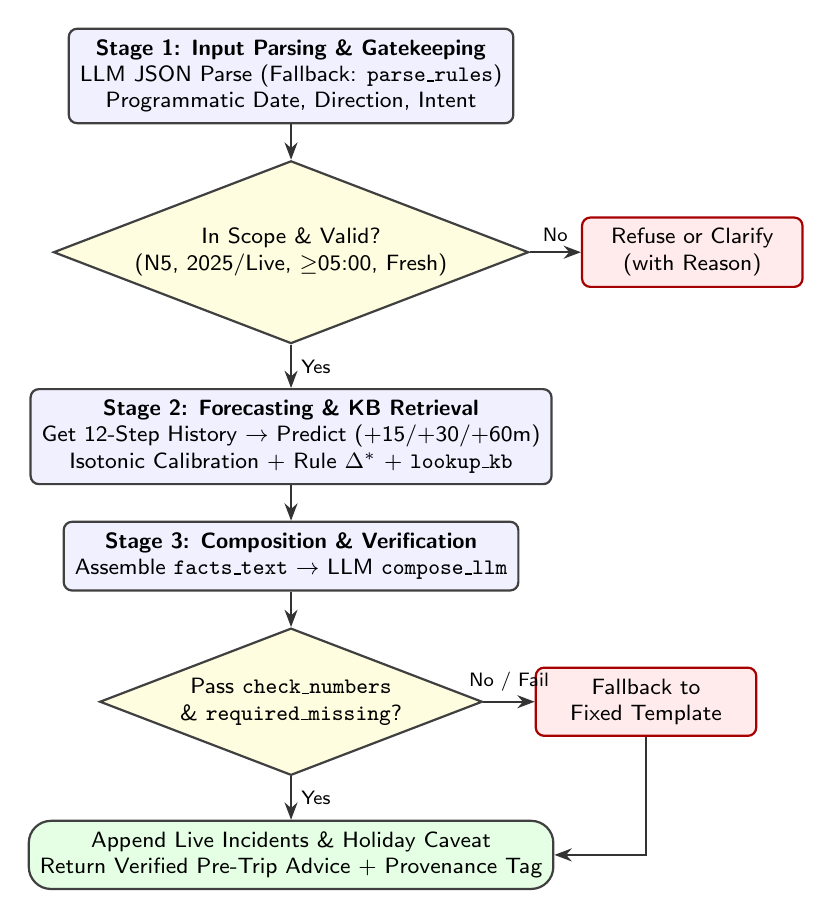
\begin{tikzpicture}[
    font=\sffamily\footnotesize,
    node distance=0.45cm and 0.6cm,
    proc/.style={rectangle, rounded corners=3pt, draw=black!75, thick, fill=blue!6, align=center, minimum width=4.6cm, minimum height=0.72cm, inner sep=4pt},
    dec/.style={diamond, aspect=2.6, draw=black!75, thick, fill=yellow!12, align=center, inner sep=2pt},
    term/.style={rectangle, rounded corners=8pt, draw=black!75, thick, fill=green!10, align=center, minimum width=4.2cm, minimum height=0.68cm, inner sep=4pt},
    warn/.style={rectangle, rounded corners=3pt, draw=red!65!black, thick, fill=red!8, align=center, minimum width=2.8cm, minimum height=0.65cm, inner sep=4pt},
    arr/.style={-{Stealth[length=2.2mm]}, thick, draw=black!80}
]
\node[proc] (s1) {\textbf{Stage 1: Input Parsing \& Gatekeeping}\\LLM JSON Parse (Fallback: \texttt{parse\_rules})\\Programmatic Date, Direction, Intent};
\node[dec, below=of s1] (d1) {In Scope \& Valid?\\(N5, 2025/Live, $\ge$05:00, Fresh)};
\node[warn, right=0.65cm of d1] (ref) {Refuse or Clarify\\(with Reason)};
\node[proc, below=0.55cm of d1] (s2) {\textbf{Stage 2: Forecasting \& KB Retrieval}\\Get 12-Step History $\rightarrow$ Predict (+15/+30/+60m)\\Isotonic Calibration + Rule $\Delta^*$ + \texttt{lookup\_kb}};
\node[proc, below=of s2] (s3) {\textbf{Stage 3: Composition \& Verification}\\Assemble \texttt{facts\_text} $\rightarrow$ LLM \texttt{compose\_llm}};
\node[dec, below=of s3] (d2) {Pass \texttt{check\_numbers}\\ \& \texttt{required\_missing}?};
\node[warn, right=0.65cm of d2] (fb) {Fallback to\\Fixed Template};
\node[term, below=0.55cm of d2] (out) {Append Live Incidents \& Holiday Caveat\\Return Verified Pre-Trip Advice + Provenance Tag};

\draw[arr] (s1) -- (d1);
\draw[arr] (d1) -- node[above, font=\sffamily\scriptsize]{No} (ref);
\draw[arr] (d1) -- node[right, font=\sffamily\scriptsize]{Yes} (s2);
\draw[arr] (s2) -- (s3);
\draw[arr] (s3) -- (d2);
\draw[arr] (d2) -- node[above, font=\sffamily\scriptsize]{No / Fail} (fb);
\draw[arr] (d2) -- node[right, font=\sffamily\scriptsize]{Yes} (out);
\draw[arr] (fb.south) |- (out.east);
\end{tikzpicture}%
}
\caption{Three-stage processing flowchart incorporating scope gatekeeping, numerical-grounding verification, and deterministic template fallback.}
\label{fig:flowchart}
\end{figure}

In \textbf{Stage~1 (Input Gatekeeping)}, the LLM extracts structured slots (\texttt{road}, \texttt{origin}, \texttt{destination}, \texttt{time}), falling back to regex-based \texttt{parse\_rules} if unreachable or malformed. Dates are extracted strictly from the raw utterance to prevent fabrication; directions follow a deterministic priority (explicit directional keyword $>$ interchange mileage ordering $>$ default Taipei-side origin); and unsupported intents (full-corridor travel time or next-day optimal departure) are refused immediately. For live queries, data staleness exceeding 20 minutes or timestamps prior to 05:00 trigger explicit refusals.

In \textbf{Stage~2 (Forecasting and Knowledge Retrieval)}, the engine retrieves the preceding 12 five-minute speed intervals, verifies data sufficiency, computes multi-horizon speeds and calibrated congestion probabilities, determines the rule-based departure timing, and queries \texttt{announcements.json} for policies active at the query time or starting within 60 minutes whose listed ramp mileages fall within the target segment ($\pm 0.15$~km tolerance). Note that traffic control measures and live incidents are presented alongside---not fed into---the forecasting model, and the response explicitly states this boundary.

In \textbf{Stage~3 (Composition and Anti-Hallucination Verification)}, all verified evidence is serialized into \texttt{facts\_text}, which serves as the sole factual context for LLM narration. The generated text must pass two deterministic audits: (1)~\texttt{check\_numbers}, verifying that every numeric token appears in \texttt{facts\_text} (aside from horizon constants $\{15, 30, 60\}$), and (2)~\texttt{required\_missing}, ensuring that any recommended waiting time and active/upcoming policy start hour are preserved. Any failure triggers an immediate fallback to the deterministic template \texttt{compose}. Finally, live incident lines (within $\pm 0.5$~km segment overlap) and multi-day holiday reliability warnings are programmatically appended, tagged with \texttt{[LLM: ...]} or \texttt{[Template: reason]}.

\subsection{Mathematical Model}
\subsubsection{Live-to-Historical Slot Alignment}
Each 5-minute interval within a day is indexed by $t \in \{0, 1, \dots, 287\}$. To align real-time \texttt{ETagPairLive.xml} timestamps $t_{\text{upd}}$ with historical M05A intervals, we apply a $-3$-minute offset rule:
\begin{equation}
t_{\text{slot}}(t_{\text{upd}}) = \left\lfloor \frac{\text{minutes}(t_{\text{upd}}) - 3}{5} \right\rfloor.
\label{eq:slot_align}
\end{equation}
For example, an update timestamped 08:08 maps to slot 08:05 (covering 08:05--08:10). Across 3,418 passenger-car records on November~8, 2026, \eqref{eq:slot_align} achieved 100\% exact speed and volume agreement with archived M05A files, compared with 5\%--88\% for alternative offsets (0, $-5$, $-8$, $-10$~min).

\subsubsection{Data-Quality Masking and Congestion Definition}
Let $v_{k,t}$ and $q_{k,t}$ denote the raw median passenger-car speed (km/h) and traffic count on segment $k \in \{0,\dots,9\}$ at slot $t$. Zero-flow intervals and physically implausible outliers are masked as missing rather than zero speed:
\begin{equation}
\tilde{v}_{k,t} =
\begin{cases}
\text{NaN}, & \text{if } (v_{k,t}=0 \land q_{k,t}=0) \lor v_{k,t}\le 0 \lor v_{k,t}>150, \\
v_{k,t}, & \text{otherwise}.
\end{cases}
\label{eq:quality_mask}
\end{equation}
Missing values in $\tilde{v}_{k,t}$ are forward-filled by at most 3 consecutive steps (15~min) to yield cleaned speeds $v^*_{k,t}$. For forecast horizons $h \in \mathcal{H} = \{3, 6, 12\}$ steps ($+15, +30, +60$~min), the regression target is $y^{\text{reg}}_{k,t,h} = v_{k,t+h}$ and the binary congestion label is:
\begin{equation}
y^{\text{clf}}_{k,t,h} = \mathbb{I}\!\left(v_{k,t+h} < \tau\right), \quad \tau = 40~\text{km/h},
\label{eq:cong_def}
\end{equation}
where $\tau = 40$~km/h is an explicit project-defined operational threshold.

\subsubsection{Feature Representation and Multi-Horizon Models}
At each valid time step $t$ (requiring $\text{tod}_t \ge 60$, i.e., 05:00 or later, and no remaining NaN values across the speed history), we construct a 13-dimensional feature vector:
\begin{equation}
\mathbf{x}_{k,t} = \big[v^*_{t},\, v^*_{t-1},\, v^*_{t-2},\, v^*_{t-3},\, v^*_{t-6},\, v^*_{t-12},\, \bar{v}^{(6)}_t,\, \sigma^{(6)}_t,\, q_t,\, \text{tod}_t,\, d_{\text{cls}},\, d_{\text{pos}},\, k\big]^\top,
\label{eq:features}
\end{equation}
where $\bar{v}^{(6)}_t$ and $\sigma^{(6)}_t$ are the 6-step (30-min) rolling mean and standard deviation of $v^*$, $\text{tod}_t \in \{0,\dots,287\}$ is the time-of-day index, $d_{\text{cls}} \in \{0,1,2\}$ encodes workday, regular weekend/holiday, or multi-day holiday ($\ge 3$ consecutive off-days), $d_{\text{pos}} \in \{0,1,2,3\}$ denotes holiday position (none, first, middle, or final day), and $k$ is treated as a categorical segment identifier.

For each horizon $h \in \mathcal{H}$, a shared histogram-based gradient boosting regressor $f^{\text{reg}}_h$ and classifier $f^{\text{clf}}_h$ produce predicted speed and calibrated congestion probability:
\begin{equation}
\hat{v}_{k,t+h} = f^{\text{reg}}_h(\mathbf{x}_{k,t}), \qquad
\hat{p}_{k,t+h} = g_{h, z_{k,t}}\!\left(f^{\text{clf}}_h(\mathbf{x}_{k,t})\right),
\label{eq:predict_calib}
\end{equation}
where $z_{k,t} = \mathbb{I}\!\left(\min_{j \in \{0,\dots,5\}} \tilde{v}_{k,t-j} \ge \tau\right)$ partitions samples into currently free-flowing versus non-free-flowing regimes, and $g_{h,z}: [0,1] \to [0,1]$ is a non-decreasing isotonic regression calibrator~\cite{zadrozny2002isotonic} fitted on out-of-training H1~2025 data to correct high-probability overconfidence.

\subsubsection{Departure Rule and Numerical Grounding Audit}
Given candidate departure offsets $\Delta \in \{0, 15, 30, 60\}$~min with associated risk $p(0) = \hat{p}_{k,t+3}$ and $p(\Delta) = \hat{p}_{k,t+\Delta/5}$ for $\Delta > 0$, the deterministic departure selector chooses:
\begin{equation}
\Delta^* = \arg\min_{\Delta \in \{0,15,30,60\}} \Big(\text{round}\big(p(\Delta),\, 1\big),\; \Delta\Big),
\label{eq:depart_rule}
\end{equation}
breaking ties in favor of earlier departure. When $\max_h \hat{p}_{k,t+h} < 0.3$, the system recommends departing immediately; when $p(\Delta^*) \ge 0.6$, it reports no uncongested window within 60~min. Finally, let $\mathcal{N}(s)$ denote the set of numeric literals extracted from text $s$ (excluding leading list markers). An LLM draft $\hat{y}_{\text{LLM}}$ passes numerical verification against structured fact sheet $\mathcal{F}$ if and only if:
\begin{equation}
\mathcal{N}_{\text{bad}} = \mathcal{N}(\hat{y}_{\text{LLM}}) \setminus \Big(\mathcal{N}(\mathcal{F}) \cup \{15, 30, 60\}\Big) = \emptyset.
\label{eq:num_check}
\end{equation}

\subsection{Algorithm Design}
Algorithm~\ref{alg:agent} formalizes the end-to-end execution of the explainable freeway congestion prediction agent, explicitly detailing parsing fallback, scope/staleness gatekeeping, programmatic tool invocation, anti-hallucination verification, and deterministic caveat attachment.

\begin{algorithm}[!t]
\caption{Explainable Freeway Congestion Prediction Agent}
\label{alg:agent}
\begin{algorithmic}[1]
\Require User query $Q$, conversation state $S$, model bundle $\mathcal{M}$, calibrator $\mathcal{G}$, knowledge base $\mathcal{K}$, mode flag $\text{use\_llm}$
\Ensure Verified response $R$ with provenance tag
\State $r \gets \textsc{ParseLLM}(Q)$; \textbf{if} parse fails \textbf{then} $r \gets \textsc{ParseRules}(Q)$
\State Deterministically extract $r.\text{date}$, $r.\text{direction}$, $r.\text{intent}$ from $Q$ and merge missing carry-over fields from $S$
\If{$r.\text{intent} \in \{\text{travel\_time}, \text{best\_time}\}$ \textbf{or} $r.\text{road} \neq \text{N5}$}
    \State \Return $\textsc{Refuse}(\text{out\_of\_scope})$
\EndIf
\If{live mode requested}
    \State $(t, \text{age}) \gets \textsc{LatestLiveSlot}(\text{now})$
    \If{$t = \text{None}$ \textbf{or} $\text{age} > 20\text{ min}$ \textbf{or} $t < 60$}
        \State \Return $\textsc{Refuse}(\text{stale\_or\_overnight})$
    \EndIf
\ElsIf{$r.\text{date}$ or $r.\text{time}$ missing \textbf{or} $r.\text{direction}$ missing}
    \State \Return $\textsc{Clarify}(r)$
\ElsIf{$\text{year}(r.\text{date}) \neq 2025$}
    \State \Return $\textsc{Refuse}(\text{unsupported\_year})$
\EndIf
\State Resolve target mainline segment $k \in \{0,\dots,9\}$ (clarify if ambiguous)
\State $V_{\text{rec}} \gets \textsc{GetRecent}(k, t, n=12)$
\State Build $\mathbf{x}_{k,t}$ via \eqref{eq:quality_mask} and \eqref{eq:features}; \textbf{if} invalid \textbf{then} \Return $\text{insufficient\_data}$
\For{$h \in \{3, 6, 12\}$}
    \State Compute $\hat{v}_{k,t+h}$ and calibrated $\hat{p}_{k,t+h}$ (for $\tau=40$~km/h via \eqref{eq:cong_def}--\eqref{eq:predict_calib})
\EndFor
\State $\mathcal{P} \gets \textsc{LookupKB}(\mathcal{K}, r.\text{date}, r.\text{direction}, t, \text{km}(k))$
\State Select optimal offset $\Delta^*$ via \eqref{eq:depart_rule} and build fact sheet $\mathcal{F}$
\If{$\text{use\_llm}$}
    \State $\hat{y} \gets \textsc{ComposeLLM}(\mathcal{F}, Q)$
    \If{LLM fails \textbf{or} \eqref{eq:num_check} fails ($\mathcal{N}_{\text{bad}} \neq \emptyset$) \textbf{or} $\textsc{RequiredMissing}(\hat{y}, \Delta^*, \mathcal{P}) \neq \emptyset$}
        \State $R \gets \textsc{ComposeTemplate}(\mathcal{F})$; tag fallback reason
    \Else
        \State $R \gets \hat{y}$; tag verified LLM
    \EndIf
\Else
    \State $R \gets \textsc{ComposeTemplate}(\mathcal{F})$
\EndIf
\If{live mode}
    \State Append overlapping incidents from \texttt{LiveEvents.xml} (or unavailability notice) to $R$
\EndIf
\If{$d_{\text{cls}} = \text{multi-day holiday}$}
    \State Append fixed holiday reliability caveat to $R$
\EndIf
\State \Return $R$
\end{algorithmic}
\end{algorithm}

\section{Experiments and Discussion}

\subsection{Experimental Environment}
All data preprocessing, model training, calibration, evaluation, and unit testing (40 offline tests verifying slot alignment, zero-flow masking, refusal rules, KB filtering, numerical verification, and calibration monotonicity) were executed in Python~3.12/3.13 using \texttt{scikit-learn~1.9.1}~\cite{pedregosa2011sklearn}, \texttt{numpy~2.5.4}, \texttt{pandas~3.1.1}, and \texttt{joblib~1.6.0}. Because the forecasting backbone uses tabular histogram-based GBDT (\texttt{HistGradientBoostingRegressor} and \texttt{HistGradientBoostingClassifier} with $\texttt{max\_iter}=250$, $\texttt{learning\_rate}=0.08$, $\texttt{random\_state}=0$, and segment ID as a categorical feature), all training and inference execute on standard CPUs without requiring GPUs. For LLM-mediated query parsing and response generation, the agent connects via an OpenAI-compatible HTTP endpoint to a self-hosted \texttt{qwen/qwen3-14b} model served by LM Studio, alongside a zero-LLM template control. All code, trained models, evaluation scripts, and SHA-256-frozen test cases are maintained in an open repository for full reproducibility.\footnote{\url{https://github.com/nns2qgdq/T1-highway-congestion-agent}}

\subsection{Dataset Description}
We construct our dataset from Taiwan Freeway Bureau TDCS M05A 5-minute gantry-pair passenger-car (class~31) speed and volume archives~\cite{tdcs_m05a}, spanning approximately 6.4~GB compressed across 2024--2025 (234~MB as cleaned daily \texttt{.npz} arrays), augmented with 2026 archives and live \texttt{ETagPairLive.xml} / \texttt{LiveEvents.xml} snapshots. We restrict scope to the 10 mainline segments of National Freeway No.~5 with both endpoints on mainline gantries (\texttt{05F}) and $\ge 90\%$ daytime training-period coverage: five southbound segments ($0.0\to 5.5$, $5.5\to 28.7$, $28.7\to 30.9$, $30.9\to 43.9$, $43.9\to 49.4$~km) and five northbound segments ($5.5\to 0.1$, $28.7\to 5.5$, $30.9\to 28.7$, $43.8\to 30.9$, $52.8\to 43.8$~km).

Temporal splits strictly prevent data leakage:
\begin{itemize}
    \item \textbf{Training Set (2024)}: Full year Jan.~1--Dec.~31, 2024.
    \item \textbf{Test Set (2025)}: Full year Jan.~1--Dec.~31, 2025 (365 days: 247 workdays, 87 regular weekends/holidays, and 31 multi-day holiday days; 748,003--780,698 valid samples per horizon; 918 congestion onset events).
    \item \textbf{Strict Out-of-Sample Set (2026)}: Jan.~1--Nov.~8, 2026 (311 days unseen during model development: 206 workdays, 73 regular weekends/holidays, and 32 multi-day holiday days; 637,220--665,072 valid samples per horizon; 680 onset events, including 129 during multi-day holidays).
    \item \textbf{Probability Calibration Split}: Isotonic calibrators are fitted on H1~2025 (Jan.--Jun.~2025) and evaluated on H2~2025 (Jul.--Dec.~2025) and 2026.
\end{itemize}

Day types are derived solely from 2024--2026 Taiwan government office calendars (never inferred from cached file availability). The regulatory knowledge base contains 43 curated entries (33 from official government pages/press releases and 10 media-relayed summaries with verbatim quotes and explicit provenance tags).

\subsection{Evaluation Metrics}
We evaluate the system across five complementary dimensions:
\begin{enumerate}
    \item \textbf{Speed Prediction Error}: Mean Absolute Error (MAE, in km/h) stratified by horizon ($+15, +30, +60$~min) and day type, comparing GBM against \emph{Persistence} ($\hat{v}_{t+h} = v_t$) and \emph{Historical Average} (training-period mean by day type, slot, and segment). Because 5-minute observations within the same day are strongly autocorrelated, all 95\% confidence intervals (CIs) for MAE and paired differences ($\Delta\text{MAE} = \text{MAE}_{\text{GBM}} - \text{MAE}_{\text{Persist}}$) are computed via \emph{day-level clustered bootstrap resampling}.
    \item \textbf{Event-Level Congestion Early Warning}: Per-sample ROC-AUC is dominated by sustained free-flow or already-congested intervals. We therefore define ground-truth \emph{onset events} as transitions from $\ge 40$ to $< 40$~km/h following at least 30~min of free flow (05:00--22:00). Alerts are permitted only when the segment is currently free-flowing (past 30~min $\ge 40$~km/h) and merged within 30~min. Thresholds are tuned per method to match three fixed alert budgets ($0.25, 0.50, 1.00$ alerts/segment/day), measuring \emph{Detection Rate} (fraction of onset events preceded by an alert within 60~min) and \emph{Precision} (fraction of alerts followed by an event within 60~min). We also evaluate an experimental \emph{Onset Model} trained exclusively on free-flowing samples to predict whether speed drops below 40~km/h within 60~min, gated by a pre-registered deployment rule requiring its 95\% CI lower bound over persistence to exceed zero at both 0.25 and 0.50 budgets in 2025.
    \item \textbf{Probability Calibration}: Expected Calibration Error (ECE), Brier Score, and high-risk calibration gap $|\bar{\hat{p}} - \bar{y}|$ on currently free-flowing samples with $\hat{p} \ge 0.3$ (pre-registered criterion: gap $\le 0.10$ across all three horizons on H2~2025).
    \item \textbf{Observation Delay Sensitivity}: Full-year 2025 MAE under simulated 0, 5, 10, and 15~min ingestion delays without model retraining.
    \item \textbf{End-to-End Agent Reliability}: A 72-query benchmark comprising 60 SHA-256-frozen core cases (20 normal, 10 out-of-scope, 8 missing-condition, 6 direction, 10 KB announcement edge cases, 4 missing-data, 2 tool-failure) plus 12 Batch-2 cases (7 live-mode using Nov.~7--9, 2026 data, 4 open-ended phrasings, 1 holiday caveat), each executed 3 times under LLM and template modes. Automated metrics assess refusal/clarification accuracy, over-refusal rate, segment/time accuracy, numerical grounding, announcement citation, rule alignment, holiday caveat presence, 3-run consistency, LLM adoption rate, and p50/p95 latency.
\end{enumerate}

\subsection{Experimental Results}

\subsubsection{Speed Forecasting Accuracy}
Table~\ref{tab:mae_results} reports stratified speed MAE across 2025 and 2026. On workdays and regular weekends, GBM achieves statistically significant MAE reductions over Persistence at every horizon in both years (all 95\% CIs strictly below zero). On workdays at $+60$~min, GBM reduces MAE from 3.771 to 3.024~km/h in 2025 ($\Delta = -0.747$) and from 3.662 to 3.113~km/h in 2026 ($\Delta = -0.549$). Historical Average performs substantially worse on weekends ($\approx 8.1$--$8.8$~km/h) and multi-day holidays ($\approx 9.9$--$10.8$~km/h) because it ignores real-time traffic states. Crucially, however, GBM's improvement over Persistence during multi-day holidays is narrow in 2025 ($-0.189$ to $-0.311$~km/h) and vanishes at $+60$~min in 2026 ($\Delta = -0.042$, 95\% CI $[-0.167, +0.079]$, crossing zero).

\begin{table*}[!t]
\caption{Speed Forecasting MAE (km/h) Across Horizons and Day Types on 2025 Test and 2026 Out-of-Sample Sets}
\label{tab:mae_results}
\centering
\footnotesize
\setlength{\tabcolsep}{4.5pt}
\begin{tabular}{llcccccccc}
\toprule
 & & \multicolumn{4}{c}{\textbf{2025 Test Year (365 Days)}} & \multicolumn{4}{c}{\textbf{2026 Out-of-Sample (311 Days)}} \\
\cmidrule(lr){3-6} \cmidrule(lr){7-10}
\textbf{Horizon} & \textbf{Day Type} & \textbf{Persist.} & \textbf{Hist. Avg.} & \textbf{GBM} & \textbf{$\Delta$MAE [95\% CI]} & \textbf{Persist.} & \textbf{Hist. Avg.} & \textbf{GBM} & \textbf{$\Delta$MAE [95\% CI]} \\
\midrule
\multirow{3}{*}{+15 min}
  & Workday   & 2.602 & 4.175 & \textbf{2.216} & $-0.386$ $[-0.396, -0.377]$ & 2.559 & 4.682 & \textbf{2.196} & $-0.363$ $[-0.375, -0.352]$ \\
  & Weekend   & 2.836 & 8.123 & \textbf{2.513} & $-0.323$ $[-0.342, -0.303]$ & 2.791 & 8.541 & \textbf{2.483} & $-0.308$ $[-0.338, -0.281]$ \\
  & Holiday   & 2.716 & 9.872 & \textbf{2.527} & $-0.189$ $[-0.227, -0.150]$ & 2.614 & 10.501 & \textbf{2.473} & $-0.141$ $[-0.184, -0.095]$ \\
\midrule
\multirow{3}{*}{+30 min}
  & Workday   & 3.030 & 4.187 & \textbf{2.556} & $-0.474$ $[-0.492, -0.456]$ & 2.963 & 4.697 & \textbf{2.560} & $-0.404$ $[-0.425, -0.381]$ \\
  & Weekend   & 3.594 & 8.196 & \textbf{3.196} & $-0.398$ $[-0.449, -0.347]$ & 3.495 & 8.614 & \textbf{3.160} & $-0.335$ $[-0.386, -0.286]$ \\
  & Holiday   & 3.374 & 9.966 & \textbf{3.192} & $-0.182$ $[-0.231, -0.135]$ & 3.231 & 10.593 & \textbf{3.174} & $-0.058$ $[-0.109, -0.010]$ \\
\midrule
\multirow{3}{*}{+60 min}
  & Workday   & 3.771 & 4.222 & \textbf{3.024} & $-0.747$ $[-0.793, -0.702]$ & 3.662 & 4.742 & \textbf{3.113} & $-0.549$ $[-0.600, -0.496]$ \\
  & Weekend   & 4.851 & 8.349 & \textbf{4.151} & $-0.701$ $[-0.814, -0.582]$ & 4.711 & 8.769 & \textbf{4.214} & $-0.497$ $[-0.615, -0.380]$ \\
  & Holiday   & 4.444 & 10.154 & \textbf{4.133} & $-0.311$ $[-0.411, -0.203]$ & 4.281 & 10.783 & 4.238 & $-0.042$ $[-0.167, +0.079]$ \\
\bottomrule
\multicolumn{10}{l}{\scriptsize Note: $\Delta\text{MAE} = \text{MAE}_{\text{GBM}} - \text{MAE}_{\text{Persist.}}$ (negative favors GBM); 95\% CIs via day-level clustered bootstrap. Bold indicates CI strictly $<0$.}
\end{tabular}
\end{table*}

\subsubsection{Event-Level Congestion Early Warning}
Although per-sample congestion ROC-AUC on 2026 data appears high (0.997 at +15~min, 0.993 at +30~min, 0.986 at +60~min; positive rate 2.6\%), Table~\ref{tab:event_results} exposes a sharply different reality under matched-budget event-level onset detection. The deployed GBM classifier underperforms simple Persistence at low and medium alert budgets in both 2025 (0.416 vs.\ 0.703 detection rate at 0.25 alerts/segment/day) and 2026 (0.263 vs.\ 0.762), and similarly lags during 2026 multi-day holidays (0.628 vs.\ 0.915 at 0.50 budget across 129 events). Training the dedicated Onset Model recovers performance to match or modestly exceed Persistence at the 0.50 budget ($+0.038$ $[+0.023, +0.053]$ in 2025; $+0.031$ $[+0.018, +0.045]$ in 2026), but its 95\% CI at the 0.25 budget crosses zero in both years ($+0.032$ $[-0.004, +0.070]$ in 2025; $+0.025$ $[-0.015, +0.062]$ in 2026) and shows zero gain on 2026 holidays ($0.000$ $[-0.047, +0.052]$ at 0.50 budget). Because it failed our pre-registered acceptance criterion, the Onset Model was deliberately not deployed into the agent.

\begin{table}[!t]
\caption{Event-Level Early Warning (Detection Rate / Precision) at Matched Alert Budgets (Alerts / Segment / Day)}
\label{tab:event_results}
\centering
\scriptsize
\setlength{\tabcolsep}{3.5pt}
\begin{tabular}{llccc}
\toprule
\textbf{Period} & \textbf{Method} & \textbf{0.25} & \textbf{0.50} & \textbf{1.00} \\
\midrule
\multirow{4}{*}{\shortstack[l]{2025 Full\\(918 events)}}
  & Persistence       & 0.703 / 0.732 & 0.911 / 0.478 & 0.958 / 0.258 \\
  & Historical Avg.   & 0.361 / 0.368 & 0.610 / 0.321 & 0.974 / 0.245 \\
  & GBM Clf. (Agent)  & 0.416 / 0.422 & 0.838 / 0.433 & 0.965 / 0.247 \\
  & Onset Model*      & 0.734 / 0.750 & 0.949 / 0.481 & 0.969 / 0.248 \\
\midrule
\multirow{4}{*}{\shortstack[l]{2026 Full\\(680 events)}}
  & Persistence       & 0.762 / 0.714 & 0.935 / 0.425 & 0.965 / 0.222 \\
  & Historical Avg.   & 0.343 / 0.394 & 0.650 / 0.295 & 0.990 / 0.221 \\
  & GBM Clf. (Agent)  & 0.263 / 0.233 & 0.825 / 0.368 & 0.978 / 0.218 \\
  & Onset Model*      & 0.787 / 0.703 & 0.966 / 0.429 & 0.984 / 0.218 \\
\bottomrule
\multicolumn{5}{l}{\scriptsize *Onset Model did not meet pre-registered criteria and was withheld from Agent.}
\end{tabular}
\end{table}

\subsubsection{Probability Calibration and Delay Sensitivity}
Unadjusted GBM probabilities exhibited severe tail overconfidence on currently free-flowing samples (e.g., on full-year 2025 $+30$~min predictions with $\hat{p} \ge 0.90$, 182 samples averaged $\bar{\hat{p}} = 0.995$ yet experienced $0.0\%$ actual congestion). Table~\ref{tab:calib_delay} shows that conditional isotonic calibration fitted on H1~2025 successfully reduced the H2~2025 high-risk gap ($|\bar{\hat{p}} - \bar{y}|$ for $\hat{p} \ge 0.3$) from 0.263 to 0.082 (+15~min), 0.165 to 0.042 (+30~min), and 0.034 to 0.028 (+60~min), passing the pre-registered $\le 0.10$ threshold at all horizons. However, on 2026 out-of-sample data, calibrated high-risk probabilities remained roughly double the realized frequency (e.g., $+30$~min: $\bar{\hat{p}} = 0.453$ vs.\ $\bar{y} = 0.237$). Under simulated observation delays (0 to 15~min on 2025 $+60$~min forecasts), GBM MAE increased modestly from 3.387 to 3.591~km/h ($\approx +0.07$~km/h per 5-minute delay), whereas Persistence degraded more sharply from 4.086 to 4.485~km/h, leaving 15-minute-delayed GBM still more accurate than zero-delay Persistence.

\begin{table}[!t]
\caption{Isotonic Calibration (Free-Flowing, $\hat{p}\ge 0.3$) and +60~min Delay Sensitivity}
\label{tab:calib_delay}
\centering
\scriptsize
\setlength{\tabcolsep}{4pt}
\begin{tabular}{lcccc}
\toprule
\multicolumn{5}{c}{\textbf{(a) H2 2025 Calibration (Free-Flowing Regime, $\hat{p} \ge 0.3$)}} \\
\midrule
\textbf{Horizon} & \textbf{Raw Gap} & \textbf{Calib. Gap} & \textbf{Brier (Raw$\to$Cal.)} & \textbf{ECE (Raw$\to$Cal.)} \\
\midrule
+15 min & 0.263 & \textbf{0.082} & 0.00340 $\to$ 0.00266 & 0.0025 $\to$ 0.0010 \\
+30 min & 0.165 & \textbf{0.042} & 0.00492 $\to$ 0.00459 & 0.0018 $\to$ 0.0010 \\
+60 min & 0.034 & \textbf{0.028} & 0.00745 $\to$ 0.00747 & 0.0011 $\to$ 0.0019 \\
\midrule
\multicolumn{5}{c}{\textbf{(b) 2025 Full-Year +60~min Speed MAE Under Observation Delay (km/h)}} \\
\midrule
\textbf{Delay} & \textbf{GBM MAE} & \textbf{Persist. MAE} & \textbf{$\Delta$MAE} & \textbf{GBM / Persist. AUC} \\
\midrule
0 min  & 3.387 & 4.086 & $-0.699$ & 0.9866 / 0.9517 \\
5 min  & 3.447 & 4.222 & $-0.775$ & 0.9854 / 0.9463 \\
10 min & 3.515 & 4.355 & $-0.840$ & 0.9841 / 0.9406 \\
15 min & 3.591 & 4.485 & $-0.895$ & 0.9826 / 0.9346 \\
\bottomrule
\end{tabular}
\end{table}

\subsubsection{End-to-End Agent Benchmark}
Table~\ref{tab:agent_eval} summarizes the 72-case (216-run per mode) agent evaluation. Both LLM-mediated and template-only modes achieved 100.0\% across every automated fidelity check---including scope refusal, zero over-refusal, exact segment/time extraction, 100\% numerical grounding, announcement citation, departure-rule compliance, holiday caveat inclusion, and 3-run consistency. Notably, in Batch~1 (60 core cases), the LLM output was accepted directly in 85.7\% of eligible runs; in the remaining 14.3\%, \texttt{check\_numbers} or \texttt{required\_missing} intercepted subtle deviations and triggered safe fallback to the deterministic template, preserving 100\% end-to-end factual fidelity. Median latency was 11.02--14.35~s for LLM mode versus 2.11--2.54~s for template mode.

\begin{table}[!t]
\caption{End-to-End Agent Evaluation Across 72 Queries (3 Runs Each)}
\label{tab:agent_eval}
\centering
\scriptsize
\setlength{\tabcolsep}{3.5pt}
\begin{tabular}{lcccc}
\toprule
 & \multicolumn{2}{c}{\textbf{Batch 1 (60 Frozen Cases)}} & \multicolumn{2}{c}{\textbf{Batch 2 (12 Live/Open)}} \\
\cmidrule(lr){2-3} \cmidrule(lr){4-5}
\textbf{Evaluation Metric} & \textbf{LLM} & \textbf{Template} & \textbf{LLM} & \textbf{Template} \\
\midrule
Refusal / Clarification Acc. (\%) & 100.0 & 100.0 & 100.0 & 100.0 \\
Over-Refusal Rate (\%)            & 0.0   & 0.0   & 0.0   & 0.0   \\
Segment \& Time Accuracy (\%)     & 100.0 & 100.0 & 100.0 & 100.0 \\
Numerical Grounding (\%)          & 100.0 & 100.0 & 100.0 & 100.0 \\
Policy Citation Accuracy (\%)     & 100.0 & 100.0 & 100.0 & 100.0 \\
Departure-Rule Consistency (\%)   & 100.0 & 100.0 & 100.0 & 100.0 \\
Holiday Caveat Included (\%)      & 100.0 & 100.0 & 100.0 & 100.0 \\
3-Run Consistency (\%)            & 100.0 & 100.0 & 100.0 & 100.0 \\
LLM Output Adopted (\%)           & 85.7  & 0.0   & 100.0 & 0.0   \\
Latency p50 / p95 (s)             & 11.02 / 24.07 & 2.11 / 8.74 & 14.35 / 20.02 & 2.54 / 8.21 \\
\bottomrule
\end{tabular}
\end{table}

\subsection{Performance Comparison}
Comparing methods across metrics underscores why multi-faceted evaluation is essential in applied ITS. First, against Historical Average, both Persistence and GBM reduce MAE by 55\%--75\% on weekends and holidays because real-time roadside conditions dominate short-horizon evolution. Second, against Persistence, GBM achieves consistent speed-MAE improvements on regular workdays and weekends across two unseen years and degrades more gracefully under 5--15~min data delays, yet offers minimal holiday benefit and no early-warning advantage for sudden congestion onset. Third, comparing LLM mode against the template baseline demonstrates that automated factual accuracy is identical (100\%) specifically because numerical reasoning and policy logic reside in deterministic tools rather than LLM weights; the LLM's contribution lies in flexible phrasing and conversational parsing, at an added p50 latency cost of $\approx 9$--$12$~s.

\subsection{Discussion}
\subsubsection{Implications of Tool-First Guardrails}
Two empirical lessons emerged during development. First, allowing an LLM to self-regulate operational disclaimers is unreliable: prior to moving holiday caveats into post-LLM programmatic attachment, \texttt{qwen/qwen3-14b} omitted the warning in 60\% of holiday runs. Second, deterministic verification (\texttt{check\_numbers} and \texttt{required\_missing}) caught 14.3\% of Batch-1 LLM drafts before reaching the user, confirming that lightweight programmatic audits are indispensable for trustworthy domain agents.

\subsubsection{Limitations}
To uphold scientific transparency, we highlight six key limitations:
\begin{enumerate}
    \item \emph{Geographic and Temporal Scope}: The agent covers only the 10 mainline segments of National Freeway No.~5 over a $\le 60$-minute horizon and does not estimate full-trip travel times or predict sudden accident-induced stoppages (TDCS M05A lacks incident features).
    \item \emph{Forecasting Ceiling on Holidays and Onset}: Holiday speed MAE gains are small and non-significant at $+60$~min in 2026, and calibrated probabilities serve as relative risk indicators rather than exact frequencies (high-risk bins remain overestimated by $\approx 2\times$ on 2026 data). Furthermore, we did not benchmark deep spatio-temporal networks (e.g., GNNs or Transformers) or external weather/event features.
    \item \emph{Unvalidated Travel-Time Impact}: The rule-based departure offset ($\Delta^*$) minimizes rounded calibrated risk, but whether following this recommendation actually reduces experienced trip travel time has not yet been empirically tested.
    \item \emph{Knowledge Base and Mapping Assumptions}: Of the 43 KB entries, 10 rely on media summaries rather than primary government pages; announcement publication timestamps, vehicle-type exemptions, and occupancy follow-up questions are not yet enforced; and ramp-to-segment mapping assumes gantry ID suffixes encode mileage $\times 10$.
    \item \emph{Live Feed Dependency}: Live-to-M05A alignment was verified across one non-holiday Sunday (3,418 records), and live mode must refuse service whenever upstream XML feeds stall beyond 20~min or return malformed event payloads.
    \item \emph{Evaluation Boundaries}: Achieving 100\% on structured automated agent cases verifies regression safety and rule enforcement rather than open-ended conversational robustness; human evaluation of clarity and decision usefulness remains to be conducted.
\end{enumerate}

\section{Conclusion}
This paper presented an explainable freeway congestion prediction agent designed to bridge the gap between raw traffic forecasting and verifiable pre-trip guidance on Taiwan's National Freeway No.~5. By treating multi-horizon HistGradientBoosting models, conditional isotonic calibrators, official traffic regulation archives, and live XML incident feeds as deterministic tools---while confining the LLM to query parsing and natural-language narration under strict numerical verification and template fallback---the proposed system eliminates unsupported numerical claims and enforces explicit scope and data-quality boundaries.

Multi-year evaluation across 2025 (365 days) and strict out-of-sample 2026 data (311 days) confirmed that GBM reliably improves short-term speed MAE over persistence on workdays ($-0.36$ to $-0.75$~km/h) and regular weekends ($-0.31$ to $-0.70$~km/h) and remains robust under 5--15~min observation delays. Equally importantly, our matched-budget event-level evaluation candidly demonstrated that multi-day holiday gains are modest and unstable, and that neither the deployed classifier nor a dedicated onset model outperforms persistence for early warning. Across 72 frozen and live-mode agent queries, deterministic verification and programmatic caveat attachment achieved 100\% numerical grounding, policy citation, and refusal accuracy. Ultimately, the system demonstrates how to deliver explainable, auditable pre-trip advice grounded in real-world ETC data---complementing rather than attempting to replace official highway services.

Future work will focus on four directions: (1)~conducting structured human evaluations to quantify explanation clarity and perceived trustworthiness relative to fixed templates; (2)~validating whether departure-timing recommendations reduce realized corridor travel times; (3)~benchmarking spatio-temporal deep learning models with exogenous weather and incident features; and (4)~extending the regulatory knowledge base with publication-time provenance checks, vehicle-occupancy follow-up dialogues, and broader national freeway coverage.

\begin{thebibliography}{00}

\bibitem{freeway2026cny}
Freeway Bureau, Ministry of Transportation and Communications (MOTC), ``2026 Lunar New Year Continuous Holiday Freeway Traffic Statistics Press Release,'' Feb.~23, 2026. [Online]. Available: \url{https://www.freeway.gov.tw/Publish.aspx?cnid=193&p=42832}

\bibitem{tdcs_m05a}
Freeway Bureau, Ministry of Transportation and Communications (MOTC), ``Traffic Data Collection System (TDCS) M05A Electronic Toll Collection Gantry Median Speed and Live XML Feeds,'' Taiwan Government Open Data. [Online]. Available: \url{https://tisvcloud.freeway.gov.tw/history/TDCS/M05A/}

\bibitem{williams2003sarima}
B.~M. Williams and L.~A. Hoel, ``Modeling and forecasting vehicular traffic flow as a seasonal ARIMA process: Theoretical basis and empirical results,'' \textit{J. Transp. Eng.}, vol.~129, no.~6, pp.~664--672, 2003.

\bibitem{wu2004svr}
C.-H. Wu, J.-M. Ho, and D.~T. Lee, ``Travel-time prediction with support vector regression,'' \textit{IEEE Trans. Intell. Transp. Syst.}, vol.~5, no.~4, pp.~276--281, Dec.~2004.

\bibitem{ke2017lightgbm}
G.~Ke, Q.~Meng, T.~Finley, T.~Wang, W.~Chen, W.~Ma, Q.~Ye, and T.-Y. Liu, ``LightGBM: A highly efficient gradient boosting decision tree,'' in \textit{Adv. Neural Inf. Process. Syst. (NeurIPS)}, vol.~30, 2017, pp.~3149--3157.

\bibitem{pedregosa2011sklearn}
F.~Pedregosa \textit{et al.}, ``Scikit-learn: Machine learning in Python,'' \textit{J. Mach. Learn. Res.}, vol.~12, pp.~2825--2830, 2011.

\bibitem{zadrozny2002isotonic}
B.~Zadrozny and C.~Elkan, ``Transforming classifier scores into accurate multiclass probability estimates,'' in \textit{Proc. 8th ACM SIGKDD Int. Conf. Knowl. Discov. Data Min. (KDD)}, 2002, pp.~694--699.

\bibitem{chen2021etc}
L.-W. Chen and D.-E. Chen, ``Exploring spatiotemporal mobilities of highway traffic flows for precise travel time estimation and prediction based on electronic toll collection data,'' \textit{Veh. Commun.}, vol.~30, Art. no.~100356, 2021.

\bibitem{zhou2021informer}
H.~Zhou, S.~Zhang, J.~Peng, S.~Zhang, J.~Li, H.~Xiong, and W.~Zhang, ``Informer: Beyond efficient transformer for long sequence time-series forecasting,'' in \textit{Proc. AAAI Conf. Artif. Intell.}, vol.~35, no.~12, 2021, pp.~11106--11115.

\bibitem{lin2024slit}
H.-T.~C. Lin, H.~Dai, and V.~S. Tseng, ``Short-term and long-term travel time prediction using transformer-based techniques,'' \textit{Appl. Sci.}, June~2024.

\bibitem{liu2024stllm}
C.~Liu, S.~Yang, Q.~Xu, Z.~Li, C.~Long, Z.~Li, and R.~Zhao, ``Spatial-temporal large language model for traffic prediction,'' in \textit{Proc. IEEE Int. Conf. Mobile Data Management (MDM)}, 2024.

\bibitem{guo2024xtpllm}
X.~Guo, Q.~Zhang, J.~Jiang, M.~Peng, M.~Zhu, and H.~Yang, ``Towards explainable traffic flow prediction with large language models,'' \textit{Commun. Transp. Res.}, 2024.

\bibitem{zhang2023trafficgpt}
S.~Zhang, D.~Fu, Z.~Zhang, B.~Yu, and P.~Cai, ``TrafficGPT: Viewing, processing and interacting with traffic foundation models,'' \textit{arXiv preprint arXiv:2309.06719}, 2023.

\bibitem{wang2024tpgpt}
B.~Wang, Z.~Cai, M.~M. Karim, C.~Liu, and Y.~Wang, ``Traffic performance GPT (TP-GPT): Real-time data informed intelligent chatbot for transportation surveillance and management,'' in \textit{Proc. IEEE 27th Int. Conf. Intell. Transp. Syst. (ITSC)}, 2024.

\bibitem{yang2025idmgpt}
F.-Z. Yang, X.~C. Liu, L.~Lu, B.-Z. Wang, and C.-X. Liu, ``Independent mobility GPT (IDM-GPT): A self-supervised multi-agent large language model framework for customized traffic mobility analysis using machine learning models,'' \textit{arXiv preprint arXiv:2502.18652}, 2025.

\end{thebibliography}

\end{document}
